
\documentclass{beamer}
\usefonttheme{structuresmallcapsserif}
\usetheme{Madrid}
\usepackage[utf8]{inputenc}
\usepackage[czech]{babel}
\usepackage{graphicx}
\usepackage[T1]{fontenc}
\usepackage{algorithm,algorithmic}
\makeatletter
\renewcommand{\ALG@name}{Algoritmus}
\makeatother

\newcommand\Omicron{O}

\title[] %optional
{Řadicí algoritmy: Bubble sort}
\subtitle{Typografie a~publikování}
\author[] % (optional)
{Jakub Valeš}

\institute[] % (optional)
{
    \href{mailto:xvales04@vutbr.cz}{xvales04@vutbr.cz}\\
}

\date[] % (optional)
{\today}


\begin{document}

\frame{\titlepage}

\begin{frame}\frametitle{Osnova}
    \begin{itemize}
        \item Motivace
        \item Přiblížení řadicích algoritmů
        \item Algoritmus Bubble sort
        \item Výhody algoritmu Bubble sort
    \end{itemize}
\end{frame}


\begin{frame}\frametitle{Motivace}
    \begin{itemize}
        \item Díky řadícím algoritmům se nám může mnoho problémů zjednodušit.
        \begin{itemize}
            \item V~seřazených seznamech se lépe hledá.
        \end{itemize}
        \item Řadící algoritmy jsou základem jiných složitějších algoritmů.
            \begin{itemize}
                \item Vyhledávací, databázové, algoritmy datových struktur.
                \item Znalost řadicích algoritmů nám pomůže tyto algoritmy pochopit.
        \end{itemize}
        \item Umožňují nám rozdělit prvky do skupin podle jejich podobností.
    \end{itemize}
\end{frame}

\begin{frame}\frametitle{Řadicí algoritmy}
    \begin{itemize}
        \item Řazení v~IT je proces uspořádávání dat do určitého pořadí.
        \item Řadicí algoritmy zajišťující \alert{uspořádání} dané sady datových záznamů \alert{do požadovaného pořadí}.
        \begin{itemize}
            \item Abecední, podle jejich velikosti (vzestupně/sestupně). 
        \end{itemize}
        \item Pro porovnávání požíváme pouze některé položky ze záznamu nazývané \alert{klíče}.
        \item Důležitými vlastnostmi těchto algoritmů jsou \alert{stabilita} a~\alert{přirozenost}.
        
    \end{itemize}
\end{frame}

\begin{frame}\frametitle{Bubble sort}
    \begin{itemize}
        \item Algoritmus několikrát prochází sadu datových záznamů a~\alert{porovnává položky vedle sebe}.
        \item V~případě že jsou položky v~nesprávném pořadí, tak je prohodí.
        \item V~případě vzestupného řazení: po prvním průchodu dostane \alert{největší prvek na poslední místo}.
    \end{itemize}
\end{frame}

\begin{frame}\frametitle{Ukázka průběhu algoritmem}
    \begin{figure}[h]
        \scalebox{0.5}{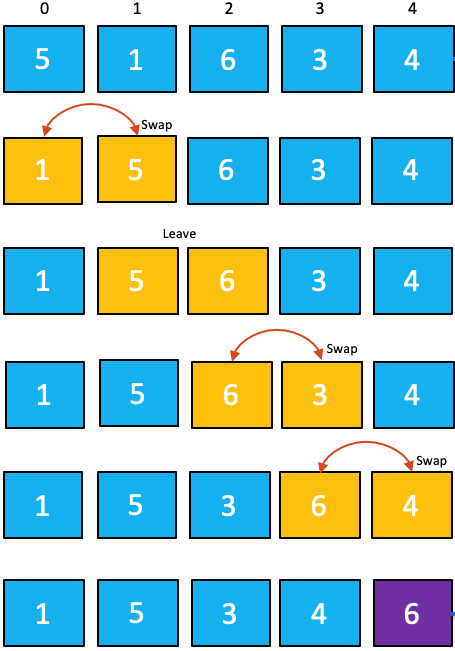
\includegraphics{bubble_sort_pass.png}}
        \caption{První iterace algoritmu Bubble sort}
        \label{obr1}
    \end{figure}
\end{frame}

\begin{frame}\frametitle{Pseudokód algoritmu Bubble sort}
    \begin{algorithm}[H]
    \hspace*{\algorithmicindent} \textbf{Input:} $A\,[MAX]$
    \begin{algorithmic}[1]
        \FOR{$i=1$ to $MAX$}
            \FOR{$j=0$ to $(MAX-1)$}
                \IF{$A\,[\,j\,] > A\,[\:j+1]$}
                    \STATE $tmp = A\,[\,j\,]$
                    \STATE $A\,[\,j\,] = A\,[\:j+1]$
                    \STATE $A\,[\:j+1] = tmp$
                \ENDIF
            \ENDFOR
        \ENDFOR
    \end{algorithmic}
    \caption{Pseudokód Bubble sort}
    \end{algorithm}
\end{frame}

\begin{frame}\frametitle{Vlastnosti algoritmu}
    \begin{itemize}
        \item Algoritmus je vhodný pro všeobecné užití.
        \item Je velmi jednoduchý na implementaci.
        \item Vhodný pro práci s~malým objemem dat.
        \item Složitost algoritmu je $\Omicron{(n^2)}$, kde $n$ představuje počet prvků
        \begin{itemize}
            \item Např. algoritmus Quicksort má složitost $\Omicron{(n \cdot \log(n))}$
        \end{itemize}
    \end{itemize}
\end{frame}

\begin{frame}\frametitle{Graf časové náročnosti Bubble sortu}
        \begin{figure}[h]
        \scalebox{0.284}{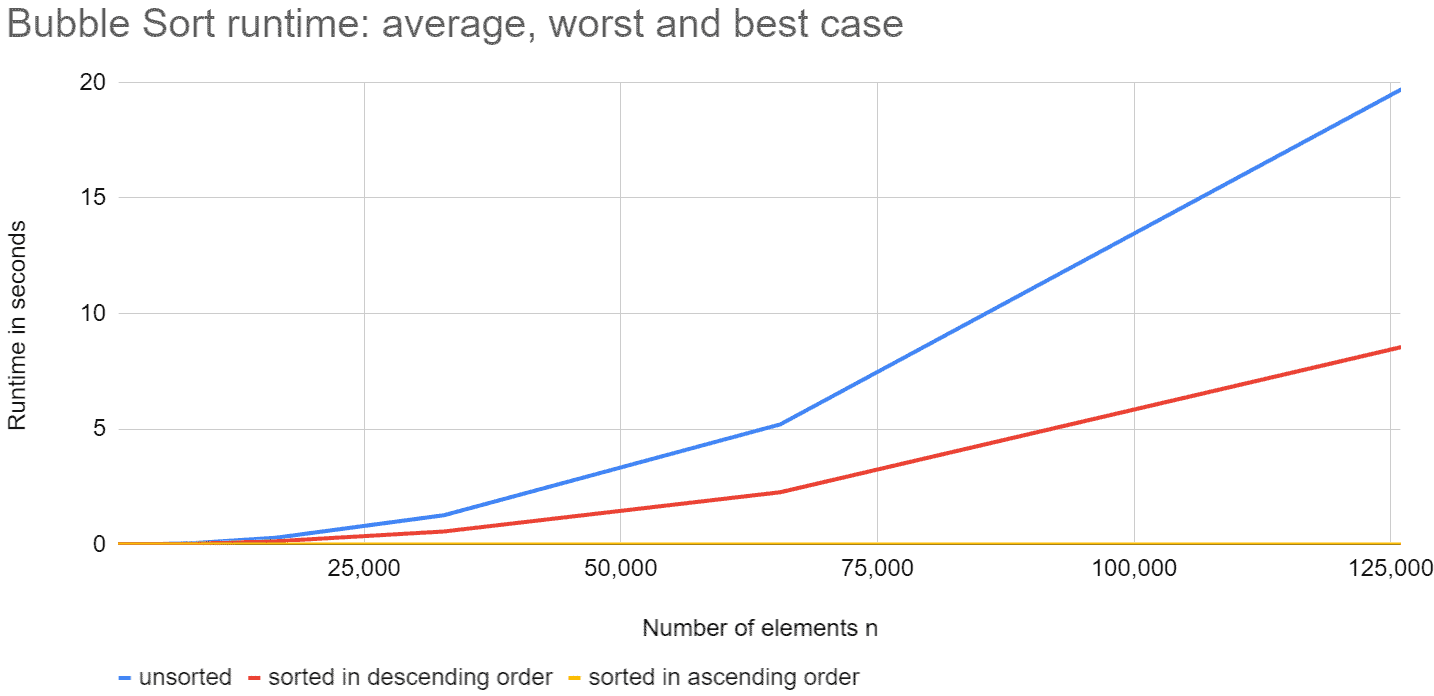
\includegraphics{Bubble_Sort_runtime.png}}
       \caption{Graf časové náročnosti algoritmu v~závislosti na počtu prvků}
        \label{obr2}
    \end{figure}
\end{frame}


\begin{frame}\frametitle{Zdroje}
    \begin{itemize}
    \transglitter
        \item Algoritmy \\ \url{https://algoritmy.net/article/75/Porovnani-algoritmu}
        \item The Sass Way \\ 
        \url{https://cutt.ly/dG4am3O/}
        \item BourneToCode \\ 
        \url{https://cutt.ly/wG4uy2F}
        \item HappyCoders \\ \url{https://happycoders.eu/algorithms/bubble-sort/}
    \end{itemize}
\end{frame}


\end{document}
